\documentclass{beamer}
\usepackage[utf8]{inputenc}
\usepackage[]{hyperref}
\usepackage{booktabs}
\usetheme[pageofpages=of,bullet=square,
	titleline=true,
	alternativetitlepage=true,
	titlepagelogo=figs-slides/xkcd-generalization2.jpg]{Torino}

\author{Statistical Reasoning\\and Quantitative Methods}
\title{Estimation}
\institute{François Briatte \& Ivaylo Petev}
\date{Session 5}

\include{beameradditions}

\begin{document}

	\begin{frame}[t,plain]
		\titlepage
	\end{frame}

	\begin{frame}[t]{Outline}
		The properties of the standard normal distribution allow for statistical \red{inference}: the \red{estimation}, at a certain level of \red{confidence}, of the unobserved \red{population} parameters, using observed \red{sample} parameters.\\[1em]
		
		But first…
		
		\begin{columns}[T]
		\column{.35\textwidth}
			\tableofcontents[hideallsubsections]
		\column{.55\textwidth}
			\begin{center}
			\href{http://xkcd.com/385/}{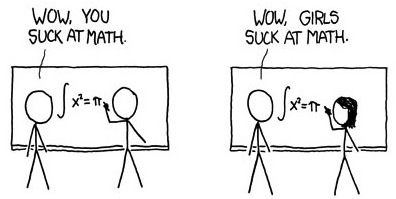
\includegraphics[scale=.4]{figs-slides/xkcd-generalization.jpg}}		
			\end{center}
		\end{columns}
	\end{frame}


	%
	%
	%
	
	\section{Assignment No. 1}
	
	%
	%
	
	\subsection{Course outline}
	
	\begin{frame}[t]{Assignment No. 1}
	
	\begin{columns}[T]
	\column{.3\textwidth}
	\textbf{Univariate\\statistics}
	
	\vspace{.55em}
	\begin{itemize}
		\item Introduction
		% (analysis of survey data)
		\item Datasets
		% (observations and variables)
		\item Distributions
		% (central tendency, variability, normality)
		\item Estimation
		% (PDF, CLT, LLN, CI, MLE)
	\end{itemize}
	\red{Assignment No. 1}\\[.5em]
	
	\fbox{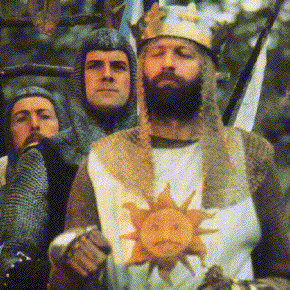
\includegraphics[width=.75\textwidth]{figs-slides/holy-grail2.jpg}}

	\column{.3\textwidth}
	\textbf{Bivariate\\statistics}
	
	\begin{itemize}
		\item Significance
		% (t-test, comparison of means and proportions)
		\item Crosstabulation
		% (Chi-squared test)
		\item Correlation
		% (scatterplot and correlation matrixes)
		\item Linear regression
		% (Simple OLS linear regression)
	\end{itemize}
	Assignment No. 2

	\column{.3\textwidth}
	\textbf{Statistical\\modelling}
	
	\begin{itemize}
		\item Basics
		% (residuals)
		\item Extensions
		% (dummies)
		\item Diagnostics
		% (multicollinearity, heteroscedasticity)
		\item Conclusion
		% (GLS, logistic, ANOVA, Bayesian...)
	\end{itemize}
	Final paper\\[.5em]
	\fbox{
\includegraphics[width=.75\textwidth]{figs-slides/holy-grail.jpg}}
	\end{columns}
	
	\end{frame}
	
	\subsection{How to proceed}
	
	% 1. Write up research design.
	% 2. Produce summary statistics.
	% 3. Replicate your work.
	
	\begin{frame}[t]{How to proceed}
	
	\textbf{First of all, complete the projects table}: \url{http://goo.gl/brYmB}\\[1em]
	
	\textbf{This table has to be complete for grading purposes}. It has to include your \red{names, class day and time, topic and dataset}.\\[1em]
	
	Then:
	
	\begin{enumerate}
		\item Write your \textbf{research design} (using the \href{http://goo.gl/7u8oa}{paper template}).
		\item Write up your do-file and export your \textbf{summary statistics}.
		\item \textbf{Replicate} your do-file and finalize your paper around \underline{3 to 5 pages}.\\[1em]
	\end{enumerate}
	
	\textbf{Finally, email us your work}, \red{copying your partner to the email}, with the email subject ``SRQM: Assignment No. 1, Briatte and Petev'' (\red{substitute your own names}). The deadline is \red{our next meeting.}
	
	\end{frame}

	\subsection{Step 1: Research design}

	% WRITE UP

	\begin{frame}[t]{Step 1: Research design}
	
	Start a text document in about \underline{2 to 4 paragraphs}:
	
	\begin{itemize}
		\item \textbf{Topic:} describe your empirical problem in the form of a \red{research question} and \red{hypotheses}.
		\item \textbf{Data:} describe your dataset with its \red{source}, \red{sample size}, \red{sampling strategy} and \red{variables}.
	\end{itemize}
	
	You can revise your hypotheses and selection of variables in future drafts. For now, stick to writing only a few paragraphs, aiming at concision (short and precise descriptions).\\[1em]
	
	The Stata Guide covers all necessary steps in Sections 1--9, with additional formatting instructions in Section 13 and a summary of instructions for this draft in Section 14.
	
	\end{frame}

	\subsubsection{Topic and dataset}
	
	\begin{frame}[t]{Topic and dataset}
		
	\begin{itemize}
		\item Your \textbf{topic} formulates a research question and derives it into testable \red{hypotheses} between your dependent and independent variables. Cite previous research if you know any.
		\item Your \textbf{dataset} is a \red{fully referenced and documented} sample for which you have read the documentation to understand what each variable measures.
	\end{itemize}
	
	Note that the total \textbf{number of observations} on which you will work at later stages might decrease because of missing data, so make sure that you are initially working on the \red{largest possible sample}.\\[1em]
	
	Use the \code{count}, \code{fre} and \code{su} commands to inspect missing data, and ignore variables for which there is an excess of missing data.
	
	\end{frame}


	\subsubsection{Variables and description}
	
	\begin{frame}[t]{Variables and description}
		
	\begin{itemize}
		\item Your \textbf{variables} have been fully \red{described}, as well as \red{renamed} and/or \red{recoded} if necessary.
		\item Your \textbf{description} of the variables is a \red{summary statistics table} with \red{additional observations} in your text. 
	\end{itemize}
	
	Note that the \textbf{number of variables} in your project is determined by your research design, and might evolve if you revise your hypotheses.\\[1em]
	
	For example, you might select something like 6 to 12 independent variables and later focus on only some of them, or even add new ones. You will also be able to revise your do-file accordingly.
	
	\end{frame}	

	
	% Topic (research question, hypotheses)
	% Data (dataset, variables)
	
	\subsection{Step 2: Summary statistics}

	\begin{frame}[t]{Step 2: Summary statistics}

	Continue with an additional \underline{2 to 4 paragraphs}:
		
	\begin{itemize}
		\item \textbf{Summary statistics:} describe all variables in a few words.
		\item \textbf{Normality:} assess how normal your dependent variable is, and describe its potential transformation.
	\end{itemize}
	
	For tables and graphs:

	\begin{itemize}
		\item The \textbf{summary statistics table} has to describe \emph{both} your \red{continuous} and \red{categorical} variables. The table is required to appear in your paper.
		
		\item The \textbf{histogram} that shows the \red{distribution of the dependent variable} can be completed by other plots showing interactions with independent variables.
	\end{itemize}
	
	\end{frame}


	\subsubsection{The tsst command}

	\begin{frame}[t]{The \code{tsst} command}
		
		\comm{Short example.}
		
		\code{use datasets/nhis2009, clear}
		
		\comm{Quick help.}
		
		\code{tsst using test.txt}
		
		\comm{Quick test.}
		
		\code{tsst using test.txt, su(age) fr(sex health) replace}\\[1em]
		
		Run \texttt{draft1.do} for a full example. Look at formatting instructions in the Stata Guide, Section 13.4, which includes an alternative to \code{tsst} if the command does not work. You can also load it manually:\\[1em]
		
		\comm{Run this line before the example above if tsst fails.}
		
		\code{run programs/tsst.ado}
	
	\end{frame}

	\subsubsection{Additional plots}

	\begin{frame}[t]{Additional plots}
		
		\begin{itemize}			
			\item The \textbf{histogram} and \textbf{diagnostic plots} that show the distribution and (ab)normality of your dependent variable are required. Also try the \code{gladder} command to find any potential transformation.

			\item \textbf{Box plots} (\code{gr box} and \code{gr hbox}), \textbf{dot plots} and \textbf{bar plots} (\code{gr dot} and \code{gr bar}) with the \code{over} option can also be used to split your dependent variable over categorical independent variables.
			
			\item \textbf{Spline plots} with the \code{spineplot} command are also recommended if you have categorical independent variables to cross-visualize.
		\end{itemize}
	
		Your plots appear only in your do-file, except if you have \emph{specific} observations to make about them. In your paper, include \underline{0 to 2 plots}.
		
	\end{frame}


	\subsection{Step 3: Replication do-file}

	\begin{frame}[t]{Step 3: Replication}
	
	Assignment No.~1 consists of:
	
	\begin{itemize}
		\item \textbf{A short paper} named in the format \code{Briatte\_Petev\_1.pdf}.
		\item \textbf{A short do-file} named in the format \code{Briatte\_Petev\_1.do}.
	\end{itemize}
	
	The do-file will include all that is needed to replicate your results: subsetting, variable renaming and recoding, summary statistics, normality tests, and tabular and graphical visualizations.\\[1em]
	
	\red{Replicate your do-file} before sending it, to make sure that it executes properly and produces the results displayed in your analysis.\\[.5em]

	\end{frame}
	
	% \subsubsection{Course do-files}
	% 
	% \begin{frame}[t]{Course do-files replication}
	% 	
	% As \red{compulsory} homework, replicate each do-file used in the course sessions, which are archived online:\vspace{.5em}
	% 						
	% 	\url{http://f.briatte.org/teaching/quanti/}
	% 
	% 	\begin{itemize}
	% 		\item Download each do-file to your \code{Replication} folder, and make sure that all course datasets are stored in the \code{Datasets} folder.
	% 		
	% 		\item Open Stata, set your working directory to the \textbf{SRQM} folder and adjust other settings as shown in \code{week1.do}.
	% 		
	% 		\item To replicate, type e.g. \code{doedit "Replication/week2.do"} and run it while reading the comments.
	% 	\end{itemize}
	% 	
	% 	(Copied from Session 3.)
	% 
	% \end{frame}
	% 
	% \begin{frame}[t]{Course do-files replication}
	% 	
	% The reason why replication is \red{compulsory} homework has to do with your learning experience throughout the course:
	% 
	% 	\begin{itemize}
	% 		\item \textbf{It helps with understanding the course session again} (or with catching up if you skipped class). You can also open the do-file in Stata and read it while replicating its commands sequentially.
	% 		
	% 		\item \textbf{It saves plain text log files in Teaching Pack $\triangleright$ Replication} that will show all comments from the do-file, along with its commands and their results.
	% 		
	% 		\item \textbf{It familiarises you with using Stata on your personal system} and contains several bits of code like commands, options and structure that can be adapted to fit your own research project.
	% 				
	% 	\end{itemize}
	% 	
	% 	Also, this is also how real-world quantitative researchers work: by reproducing each other's work, using \red{replication material}.
	% 
	% \end{frame}
	% 
	% \subsubsection{Real-world do-files}
	% 
	% \begin{frame}[t]{Real-world replication example}
	% 	
	% As \red{optional} homework, replicate economist Dani Rodrik's paper ``\textbf{The Real Exchange Rate and Economic Growth}'' (2008):\vspace{.5em}
	% 						
	% 	\url{http://www.hks.harvard.edu/fs/drodrik/research.html}
	% 
	% 	\begin{itemize}
	% 		\item Download the paper (PDF) and replication material archive (RAR) from Dani Rodrik's online research page.
	% 		
	% 		\item Open Stata and set your working directory (\code{cd}) to the folder created by decompressing the archive.
	% 		
	% 		\item Rename the do-file as \code{master.do} and run the following command in Stata: \code{do master.do, nostop}
	% 	
	% 	\end{itemize}
	% 	
	% 	Now watch the figures pop up and regression models run in the \textbf{Results} window. A few uninstalled commands and some of Dani Rodrik's personal settings will be skipped by the \code{nostop} option.
	% 
	% \end{frame}
	% 
	% \begin{frame}[t]{Real-world replication example}
	% 	
	% On my own system, I added a few tweaks that you can adapt to your own system if you want to replicate the analysis in full:
	% 
	% 	\begin{itemize}
	% 		\item After downloading all files to my Desktop, I renamed the folder to \code{rodrik2008} and the do-file to \code{master.do}.
	% 		
	% 		\item In the do-file, \code{graph export} is set to use WMF; on Mac OS X, find and replace ``\code{.wmf}'' by ``\code{.pdf}'' to export all figures.
	% 		
	% 		\item The \code{outreg2} and \code{xtabond2} packages need to be installed with \code{ssc install} to ensure that all commands will run.
	% 							
	% 	\end{itemize}
	% 	
	% 	The \code{rodrik2008} folder will contain graphs, exported tables and a log file named \code{arellano\_bond.txt} after the do-file has run.
	% 
	% \end{frame}


	% \subsubsection{Your do-file}
	% 
	% \begin{frame}[t]{Personal do-files}
	% 	
	% We will assess your research project by replicating your do-file and evaluating your analysis:
	% 
	% 	\begin{itemize}
	% 		\item \textbf{Your do-file} needs to use the appropriate commands at the right place, with some structure and comments to guide the reader.
	% 		
	% 		Try \red{replicating your own do-file} before submitting it: the code must execute properly and the results must correspond to those reported in your work.
	% 		
	% 		\item \textbf{Your text} contains the interpretation of \emph{selected} do-file results: without a proper do-file, you will struggle to produce any accurate analysis.
	% 		
	% 		Valid statistical reasoning needs \textit{much} more than a do-file, but \red{correct, comprehensible code} is a prerequisite to writing up a coherent quantitative paper.
	% 							
	% 	\end{itemize}
	% 		
	% \end{frame}
	
	
	% \subsubsection{Your code}
	% 
	% \begin{frame}[t]{Your code}
	% 	
	% We will assess your research project by replicating your do-file and evaluating your analysis:
	% 
	% 	\begin{itemize}
	% 		\item \textbf{Your do-file} needs to use the appropriate commands at the right place, with some structure and comments to guide us through your work.
	% 		
	% 		Try \red{replicating your own do-file} before submitting it: the code must execute properly and the results must correspond to those reported in your work.
	% 		
	% 		\item \textbf{Your text} contains the interpretation of (some of) the do-file results: without a proper do-file, you will struggle to produce any accurate analysis.
	% 		
	% 		Valid statistical reasoning needs \textit{much} more than a do-file, but \red{correct, comprehensible code} is a prerequisite to writing up a coherent quantitative paper.
	% 							
	% 	\end{itemize}
	% 		
	% \end{frame}
	
	\subsection{Further help}
	
	\begin{frame}[t]{Further help}

		\begin{itemize}

			\item Course-specific help:

			\begin{itemize}
				\item Stata Guide
				\item Session do-files
				\item Course slides
			\end{itemize}
	
			\item General help:
			
			\begin{itemize}
				\item Handbook chapters
				\item Stata documentation (\code{help \emph{command}})
				\item Online tutorials
			\end{itemize}

		\end{itemize}

		Everything is systematically archived on the course website:\\[.5em]
		
		\url{http://f.briatte.org/teaching/quanti/}\\[.5em]
		
		Happy coding!
		
	\end{frame}

	%
	%
	%

	\begin{frame}[t,plain]
		
		\vspace{.4\textheight} 
		And now, estimation.
		
		\begin{flushright}
		\includegraphics[scale=.3]{figs-slides/longcat.jpg}		
		\end{flushright}
	\end{frame}
		
	\section{Estimation}

	%
	%
	%
	
	\begin{frame}[t]{Standard normal distribution $\mathcal{N}(0,1)$}
	
	\begin{itemize}
		\item $\mu \pm 1\sigma$ contains approximately \textbf{68\%} of all values.
		\item $\mu \pm 2\sigma$ contains approximately \textbf{95\%} of all values.
		\item $\mu \pm 3\sigma$ contains approximately \textbf{99\%} of all values.
	\end{itemize}
	
	\begin{center}
		\href{http://en.wikipedia.org/wiki/Normal_distribution}{\includegraphics[scale=.5]{figs-slides/normal-distr.pdf}}
	\end{center}
		
	\end{frame}

	\begin{frame}[t]{Probability density function}
	
	\begin{itemize}
		\item $Pr(\mu - 1\sigma < \mu < \mu + 1\sigma) \approx .68$
		\item $Pr(\mu - 2\sigma < \mu < \mu + 2\sigma) \approx .95$
		\item $Pr(\mu - 3\sigma < \mu < \mu + 3\sigma) \approx .99$
	\end{itemize}
	
	\begin{center}
		\href{http://en.wikipedia.org/wiki/Normal_distribution}{\includegraphics[scale=.5]{figs-slides/normal-distr.pdf}}
	\end{center}
		
	\end{frame}
		
	\begin{frame}[t]{Estimation}

	The normal distribution is used for \red{statistical inference}, i.e. for estimating the \red{population} parameters from the \red{sample} parameters.\vspace{1em}

\begin{center}
\begin{tabular}{lcc}
	\toprule
	& \multicolumn{2}{c}{Notation} \\
	\cmidrule(r){2-3}
	Parameter & \red{Sample} & \red{Population} \\
	\midrule
	Mean & $\bar X$ & $\mu$ \\
	Standard deviation & $s$ & $\sigma$ \\
	\bottomrule
\end{tabular}
\end{center}
	\vspace{1em}
	
	This operation \red{generalizes} the values held by the sample to the population under consideration, under certain \red{levels of confidence}.

	\end{frame}
	
	\fullslide{figs-slides/bigbangtheory-equations.jpg}

	%
	
	\subsection{Central Limit Theorem}
		
	\begin{frame}[t]{Central Limit Theorem}

	Formally, $\mu$ is the \red{population mean}, which is unobserved, and $\bar{X}$ is the \red{sample mean}, which is observable by analysing the data.\vspace{1em}

The \textbf{Central Limit Theorem} (CLT) states that, if repeated samples are drawn from the population, their respective means $\bar X_1, \bar X_2,... , \bar X_n$ will be \red{normally distributed} around the population mean $\mu$:

		$$\textsf{CLT}: \sqrt{N}\bigg(\frac{1}{N}\sum_{i=1}^N \bar X_i - \mu\bigg)\ \xrightarrow{d}\ \mathcal{N}(0,\;\sigma^2)$$
		
		\vspace{1em}
		\begin{columns}[T]
		\column{.625\textwidth}
		The CLT holds \red{regardless of the distribution} of the variable $X$ under examination, which is, like, totally awesome.
		\column{.3\textwidth}
		\vspace{1.5em}
		\begin{flushright}
		\includegraphics[scale=.3]{figs-slides/longcat.jpg}		
		\end{flushright}
		\end{columns}
	\end{frame}

	%
	
	\subsection{Law of Large Numbers}

	\begin{frame}[t]{Law of Large Numbers}

	Formally, $\sigma$ is the \red{population standard deviation}, which is unobserved, and $s$ is the \red{sample standard deviation}, which is observable by analysing the data.\vspace{1em}

The \textbf{Law of Large Numbers} states that, the larger the sample, the closer its mean will be to the population mean. The \red{standard error} of that estimate derives from the standard deviation of the variable.\vspace{1em}

The \red{standard error of the mean} (SEM), which estimates the standard deviation of the population from the standard deviation in the sample, will hence (slowly) decrease with sample size:

\vspace{1em}

		\begin{columns}[T]
		\column{.625\textwidth}
		$$\textsf{SEM} = SE_{\bar X} = \frac{s}{\sqrt{N}}~\textsf{(sample)}$$
		\column{.3\textwidth}
		\begin{flushright}
		\vspace{-4em}
		\includegraphics[scale=.3]{figs-slides/longcat.jpg}		
		\end{flushright}
		\end{columns}
	\end{frame}

	%
	
	\subsection{Confidence intervals}
		
	\begin{frame}[t]{Confidence intervals}

	Given these properties, the population mean $\mu$ can be estimated from a sample $X$ of $N$ (statistically independent) observations.\vspace{1em}

%	\begin{itemize}
%		\item 
		\textbf{When we observe a normal distribution}, $\mu \pm 2\sigma$ contains approximately 95\% of all values. The exact number used for estimation at \red{95\% confidence}, called the \red{z-score}, is $z = 1.96$.\\
		\vspace{1em}
%		\item 
\textbf{When the sample values of $X$ are normally distributed}, $\bar X \pm 1.96 \cdot SE_{\bar X}$ contains 95\% of the possible values of $\mu$.\\[1em]

These bounds define a \red{95\% confidence interval}:

%	\end{itemize}

	\begin{columns}[T]
		\column{.625\textwidth}
		\hspace{.725em}
		$\bar{X} -1.96 \cdot SE_{\bar X} < \mu < \bar{X} + 1.96 \cdot SE_{\bar X}$	
		\begin{itemize}
%			\item In 95\% of cases, $\bar{x} -1.96 \cdot SE_{\bar x} < \mu < \bar{x} + 1.96 \cdot SE_{\bar x}$.
			\item In 2.5\% of cases, $\mu < \bar{X} - 1.96$.
			\item In 2.5\% of cases, $\mu > \bar{X} + 1.96$.					\end{itemize}
		\column{.3\textwidth}
		\vspace{-4em}
		\begin{flushright}
		\includegraphics[scale=.3]{figs-slides/longcat.jpg}		
		\end{flushright}
	\end{columns}

%	Estimation of population parameters is possible only when the properties of the normal distribution are present in the data.
	
	\end{frame}
	
	\begin{frame}[t]{Stata implementation}
			
	%\includegraphics[width=\textwidth]{figs-slides/ci.pdf}
	
	Summary statistics for current worldwide fertility rates:\\
	\code{su births}\\[1em]
	
	\includegraphics[width=\textwidth]{figs-slides/ci1.pdf}\\[1em]
	
%	Pocket calculator approach: \code{di 1.64/sqrt(186), 3.13-1.96*(1.64/sqrt(186)), 3.13+1.96*(1.64/sqrt(186))}

%$	$$\red{SE_{\bar X}} \approx \frac{1.64}{\sqrt{186}}\approx 0.12\hspace{1em}	\red{\textsf{95\% CI}} \approx 3.13 \pm 1.96 \cdot 0.12 \approx \red{[2.89,3.36]}$$

	Standard error and 95\% confidence interval:\\
	\code{ci births}\\[1em]
	
	\includegraphics[width=\textwidth]{figs-slides/ci2.pdf}\\[1em]
	
	\begin{itemize}
		\item Use the \code{level(99)} option for a \red{larger} 99\% confidence interval.
		\item Use the \code{binomial} option if the variable is \red{dichotomous} (binary).
	\end{itemize}	
	\end{frame}

	\begin{frame}[t]{Stata implementation: Q\&A}
			
	%\includegraphics[width=\textwidth]{figs-slides/ci.pdf}
	
	\begin{itemize}
		\item \textbf{Q: Why is the 99\% confidence interval larger?}\\[.25em]
		
		A: The 99\% CI uses $z = 2.58$ to include 99\% of all possible values of $\mu$ in the interval. Its calculation with $\bar X \pm 2.58 \cdot SE_{\bar X}$ therefore includes more values on both sides of $\bar X$.\\[.25em]
		
		This is called the \red{precision-accuracy trade-off}: higher confidence for $\mu$ is obtained at the expense of a more precise value for $\mu$. \red{Maximising sample size} will attenuate the trade-off.\\[.25em]
		
		\item \textbf{Q: Why do we apply a `binomial' option to binary variables?}\\[.25em]
		
		A: Binary outcomes of ``yes/no'' variables form a distribution with no intermediate values that cannot be normal. Instead, the discrete probability of independent 0/1 outcomes (\red{Bernoulli trials}) is given by the \red{binomial distribution}.\\[.25em]
		
		We will focus on estimation based on the normal distribution.
	\end{itemize}
		
%	Pocket calculator approach: \code{di 1.64/sqrt(186), 3.13-1.96*(1.64/sqrt(186)), 3.13+1.96*(1.64/sqrt(186))}

%$	$$\red{SE_{\bar X}} \approx \frac{1.64}{\sqrt{186}}\approx 0.12\hspace{1em}	\red{\textsf{95\% CI}} \approx 3.13 \pm 1.96 \cdot 0.12 \approx \red{[2.89,3.36]}$$

	\end{frame}

	%
	
	\subsection{Back to Estimation}
		
	\begin{frame}[t]{Back to estimation}
	
	Using the normal distribution as a probability density function and standardised $z$-scores to select a level of confidence:
		
	\begin{columns}[T]
	
	\column{.625\textwidth}
	\vspace{-.5em}
	\begin{center}
	\begin{tabular}{lcc}
		\toprule
		& \multicolumn{2}{c}{Notation} \\
		\cmidrule(r){2-3}
		Parameter & \red{Sample} & \red{Population} \\
		Observations & $N$ & unobserved \\
		\midrule
		Mean & $\bar X$ & $\mu$\\
		Standard deviation & $s$ & $\sigma$ \\
		\red{Standard error} & $SE$ & \\
		\bottomrule
	\end{tabular}\\[1em]
	Estimating $\mu$ at 95\% or 99\% confidence:\\[.5em]
	$Pr(\mu \in \bar X \pm z = 1.96 \cdot SE_{\bar X}) = .95$\\	
	$Pr(\mu \in \bar X \pm z = 2.58 \cdot SE_{\bar X}) = .99$
	\end{center}

	\column{.3\textwidth}
	\vspace{4em}
	\begin{flushright}
	\includegraphics[scale=.3]{figs-slides/longcat.jpg}		
	\end{flushright}
		
	\end{columns}
	\end{frame}

	\begin{frame}[t]{Back to estimation}

	For a variable $X$, estimating $\mu$ from $\bar X$ relies on three prerequisites that you will apply to all your variables:

	\begin{itemize}
		\item \textbf{Assess the distribution}'s \red{normality} i.e. whether $X \sim \mathcal{N}(\mu,\sigma)$.
		\item \textbf{Select the standardised $z$-score} to fix a \red{level of confidence}.
		\item \textbf{Minimise the sampling error} by maximising the \red{sample size} ($N$).
	\end{itemize}
	
	\begin{columns}[T]
	
	\column{.625\textwidth}

	This technique guides all \red{point estimation} that we perform in this course. It is called \red{Maximum Likelihood Estimation} (MLE).\\[1em]
	
	Following the assumptions of MLE pleases \textbf{Estimation Cat}, the first of two cats in The Prophecy.
	\column{.3\textwidth}
	\vspace{0em}
	\begin{flushright}
	\includegraphics[scale=.3]{figs-slides/longcat.jpg}		
	\end{flushright}
		
	\end{columns}
		
	\end{frame}

	%
	%
	%
	
	\section*{The Prophecy}
	
	%
	%
	%
		
	\begin{frame}[t]{The Prophecy}

	The Prophecy states that the powers of Estimation Cat (white) are limited by those of \textbf{Significance Cat} (black).

	\begin{itemize}
		\item \textbf{Estimation} provides a parameter and its \red{standard error}. Relationships between variables can be modelled as parameters.
		\item \textbf{Statistical significance} provides its \red{probability level}, i.e. the probability that the estimated parameter is different from zero.
	\end{itemize}
	
	\vspace{.5em}
	
	\begin{columns}[T]
	
	\column{.625\textwidth}

	\textbf{Parametric statistics} work by confronting the awesome powers of Estimation Cat and Significance Cat into a \red{model}.\\[1em]
	
	This course is an introduction to statistical modelling using frequentist statistics, a.k.a The Prophecy.
	\column{.3\textwidth}
	\vspace{0em}
	\begin{flushright}
	
\includegraphics[scale=.3]{figs-slides/longcat-black.jpg}		
	\end{flushright}
		
	\end{columns}
		
	\end{frame}
	
	% We use Estimation Cat and Significance Cat to keep them from
	% getting bored and taking over the world. That's the Prophecy.
	
	\fullslide{figs-slides/longcat-prophecy.jpg}
	
\end{document}